% Chapter: 02_llm_steganography
% Included from lectures/steganography/main.tex

\section{Steganography with LLMs}

\newcommand{\llmstegodiagram}[1]{%
\begin{tikzpicture}[
  box/.style={rectangle, draw, thick, rounded corners=3pt, minimum height=0.65cm, minimum width=1.95cm, font=\small, align=center},
  op/.style={box, fill=blue!15},
  data/.style={box, fill=green!15},
  side/.style={box, fill=orange!15},
  plain/.style={box, fill=gray!15, minimum width=2.7cm},
  arr/.style={->, very thick, gray!70},
  group/.style={rectangle, draw, dashed, gray, rounded corners=5pt, inner sep=5pt},
]
  \node[data] (m) at (0, 0) {payload $m$};
  \node[op] (enc) at (2.6, 0) {Encrypt};
  \node[data] (x) at (2.6, -0.95) {ciphertext $x$};
  \node[op] (emb) at (2.6, -1.9) {Embed};
  \node[data] (s) at (5.8, -1.9) {stegotext $s$};
  \node[op] (ext) at (9.0, -1.9) {Extract};
  \node[data] (x2) at (9.0, -0.95) {ciphertext $x$};
  \node[op] (dec) at (9.0, 0) {Decrypt};
  \node[data] (m2) at (11.6, 0) {payload $m$};
  \node[side] (key) at (5.8, 0) {secret key $k$};
  \node[side] (llm) at (5.8, -0.95) {LLM logits};
  \node[box, fill=red!15] (w) at (5.8, -2.9) {Warden};
  \node[plain] (is) at (2.6, -3.9) {LLM};
  \node[data] (c) at (5.8, -3.9) {covertext $c$};
  \node[plain] (ir) at (9.0, -3.9) {Innocent receiver};

  \begin{scope}[on background layer]
    \node[group, fit=(enc)(x)(emb), label={[font=\scriptsize, gray]above:Sender}] (snd) {};
    \node[group, fit=(ext)(x2)(dec), label={[font=\scriptsize, gray]above:Receiver}] (rcv) {};
  \end{scope}

  \draw[arr] (m) -- (enc);
  \draw[arr] (enc) -- (x);
  \draw[arr] (x) -- (emb);
  \draw[arr] (emb) -- (s);
  \draw[arr] (s) -- (ext);
  \draw[arr] (ext) -- (x2);
  \draw[arr] (x2) -- (dec);
  \draw[arr] (dec) -- (m2);
  \draw[arr] (key) -- (key -| snd.east);
  \draw[arr] (key) -- (key -| rcv.west);
  \draw[arr] (llm) -- (llm -| snd.east);
  \draw[arr] (llm) -- (llm -| rcv.west);
  \draw[arr] (is) -- (c);
  \draw[arr] (c) -- (ir);
  \draw[arr, dashed] (s) -- (w);
  \draw[arr, dashed] (c) -- (w);
  \node[font=\scriptsize, right, align=left] at (w.east) {what is $m$? \\ do I see $s$ or $c$?};
  #1
\end{tikzpicture}%
}

\begin{frame}{Steganography with LLMs}
\begin{center}
\llmstegodiagram{}
\end{center}

\note{
\begin{itemize}
\item The same picture as in the theory part, with two changes
\item The innocent sender is an LLM: covertext is a normal response of the model
\item Sender and receiver share more than the key, both have access to the LLM's logits
\item So both know the covertext distribution exactly, token by token
\item The stegotext has to look like a normal response of the same LLM
\item Later: a scheme where the receiver does not need the logits
\end{itemize}
}
\end{frame}

\begin{frame}{Perfect Security with LLMs: Coupling}
\begin{itemize}
\item \textbf{Theorem 1}: $f$ is perfectly secure iff it samples $S$ from row $x$ of a \textbf{coupling}, a joint table over $(X, C)$ with row sums $X$ and column sums $C$
\item \textbf{Theorem 2}: the coupling with maximal $I(X; S)$ is the one with \textbf{minimum joint entropy} $H(X, S)$ (MEC)
\end{itemize}

\source{dewitt2022}

\note{
\begin{itemize}
\item This is the perfectly secure counterpart to the PRF scheme that follows
\item It uses Cachin's model: everyone, including the warden, knows the covertext distribution exactly
\item Step 1 is the one-time pad from the theory part, the key is as long as the payload
\item Theorem 1 is almost a tautology: the stegotext marginal equals the covertext distribution exactly when the joint is a coupling
\item Theorem 2: $I(X; S) = H(X) + H(S) - H(X, S)$, $H(X)$ is fixed and $H(S) = H(C)$ by perfect security, so maximising information means minimising the joint entropy
\item So the question ``what is the best perfectly secure scheme'' becomes ``find the minimum entropy coupling''
\end{itemize}
}
\end{frame}

\begin{frame}{Minimum Entropy Coupling: Greedy Construction}
\begin{center}
\foreach \n in {1,...,12}{\only<\n>{\includegraphics[height=0.8\textheight]{figures/mec_steps/step_\n.pdf}}}
\end{center}

\note{
\begin{itemize}
\item Rows: the four ciphertexts, each with probability mass $0.25$
\item Columns: the three tokens with the LLM's probabilities
\item The strips on the right and at the bottom show the mass that is still left per ciphertext and per token
\item Second step: the independent coupling, every cell is the product of its row and column mass
\item It has the right row and column sums, so it is perfectly secure, but the token says nothing about $x$, it is useless
\item Then start again from the empty table
\item Greedy rule (Kocaoglu et al.\ 2017): take the ciphertext with the most mass left and the token with the most room left, move the minimum of the two
\item Repeat until all mass is placed
\item Every column sums to the token probability, so the token distribution is unchanged
\item Reading a column gives the receiver's posterior: \texttt{fox} means $x = 11$ for sure, \texttt{dog} means $01$ with probability $5/6$, \texttt{cat} leaves $00$ and $10$ equally likely
\item Exact MEC is NP-hard, but greedy approximations are within about one bit of optimal and keep the marginals exact
\item The toy example is my own, not from the paper
\end{itemize}
}
\end{frame}

\begin{frame}{iMEC: Coupling Token by Token}
Ciphertext and text are far too large for one coupling table, so couple step by step.
\begin{columns}[T]
\begin{column}{0.42\textwidth}
\begin{itemize}
\item Keep a posterior $\mu$ over the ciphertext (start: uniform)
\item Each token $j$: couple $\mu$ with the LLM's next-token distribution, sample $S_j$, update $\mu$ to the posterior given $S_j$
\item The receiver runs the same computation and ends with the MAP ciphertext
\item Stop once $H(\mu) < 0.1$ bits
\end{itemize}
\end{column}
\begin{column}{0.56\textwidth}
\includegraphics[width=\textwidth]{figures/imec_posterior.pdf}
\end{column}
\end{columns}

\source{dewitt2022}

\note{
\begin{itemize}
\item iMEC is from Sokota et al.\ 2022, de Witt et al.\ apply it to steganography
\item The ciphertext is split into blocks, each step couples the block with the highest remaining entropy
\item Every step is a coupling, so every token has exactly the LLM's distribution, perfect security holds for the whole text
\item The plot is my own toy simulation: each line is one run, the receiver's uncertainty falls roughly by the entropy of each token
\item The receiver needs the exact same next-token distributions as the sender: the same model, the same prompt, deterministic numerics
\end{itemize}
}
\end{frame}

\begin{frame}{Find a scheme that works without giving the receiver access to the LLM}
\begin{center}
\llmstegodiagram{
  \path (llm.east) -- (llm -| rcv.west) coordinate[midway] (cut);
  \draw[red, line width=2.5pt] ($(cut)+(-0.22,-0.22)$) -- ($(cut)+(0.22,0.22)$);
  \draw[red, line width=2.5pt] ($(cut)+(-0.22,0.22)$) -- ($(cut)+(0.22,-0.22)$);
}
\end{center}
\end{frame}

\begin{frame}{PRF + LLM = Undetectable Steganography}
\begin{center}
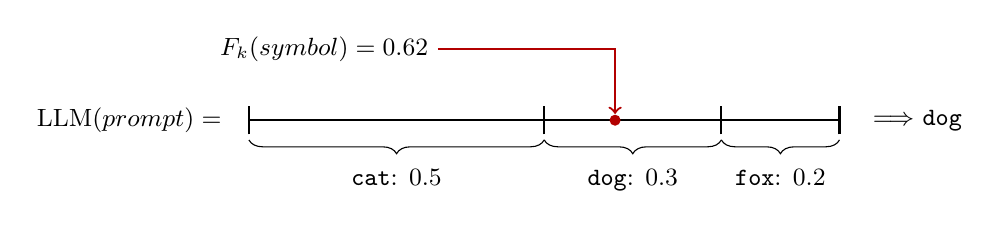
\begin{tikzpicture}[
  x=0.75cm,
  y=1cm,
  font=\small,
  tokenbrace/.style={decorate, decoration={brace, mirror, amplitude=5pt}},
]
  \draw[thick] (0, 0) -- (10, 0);
  \foreach \x in {0, 5, 8, 10}
    \draw[thick] (\x, -0.18) -- (\x, 0.18);

  \draw[tokenbrace] (0, -0.25) -- (5, -0.25) node[midway, below=7pt] {\texttt{cat}: $0.5$};
  \draw[tokenbrace] (5, -0.25) -- (8, -0.25) node[midway, below=7pt] {\texttt{dog}: $0.3$};
  \draw[tokenbrace] (8, -0.25) -- (10, -0.25) node[midway, below=7pt] {\texttt{fox}: $0.2$};

  \node[anchor=east] at (-0.3, 0) {$\mathrm{LLM}(\text{prompt}) =$};
  \node[anchor=east] (prf) at (3.2, 0.9) {$F_k(\text{symbol}) = 0.62$};
  \draw[thick, ->, red!70!black] (prf.east) -- (6.2, 0.9) -- (6.2, 0.08);
  \fill[red!70!black] (6.2, 0) circle (2pt);
  \node[anchor=west] at (10.4, 0) {$\Longrightarrow$ \texttt{dog}};
\end{tikzpicture}
\end{center}
\vspace{-0.3em}
\begin{itemize}
\item Normal sampling: draw a uniform $u \in [0, 1]$ and pick the token whose interval contains $u$
\item Steganography: replace $u$ by the output of a secret-keyed PRF that depends on the payload symbol
\item The PRF output looks uniform, so the token distribution is unchanged
\item Any signal with entropy can be turned into a stego channel this way
\end{itemize}

\source{zamir2024}

\note{
\begin{itemize}
\item At every step the language model produces a probability distribution over the next token
\item Example: cat $0.5$, dog $0.3$, fox $0.2$
\item Normally the model samples a random number $u$ and chooses the token by cumulative probability intervals: cat if $u < 0.5$, dog if $0.5 \leq u < 0.8$, fox if $0.8 \leq u < 1$
\item The paper keeps this exact sampling procedure, but generates $u$ with a secret-keyed PRF instead of fresh randomness
\item The model still outputs cat, dog and fox with probabilities $0.5$, $0.3$, $0.2$
\item The payload is encoded by making the PRF input depend on the payload symbol currently being transmitted
\item Sender and receiver share the PRF and the secret key $k$
\end{itemize}
}
\end{frame}

\begin{frame}{Encoding: Sampling a Token Bit by Bit}
\begin{columns}[T]
\begin{column}{0.45\textwidth}
\begin{center}
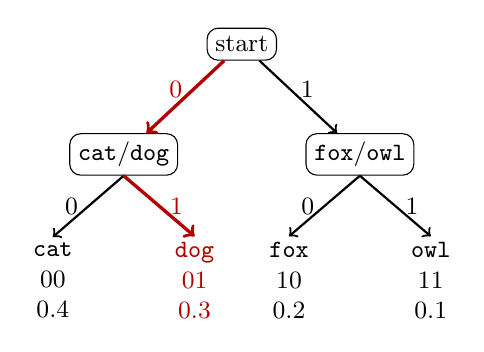
\begin{tikzpicture}[
  font=\small,
  inner/.style={draw, rounded corners, inner sep=3pt},
  leaf/.style={inner sep=2pt},
  edge/.style={thick, ->},
  chosen/.style={very thick, ->, red!70!black},
]
  \node[inner] (root) at (0, 0) {start};
  \node[inner] (l) at (-1.5, -1.4) {\texttt{cat}/\texttt{dog}};
  \node[inner] (r) at (1.5, -1.4) {\texttt{fox}/\texttt{owl}};
  \node[leaf, align=center] (cat) at (-2.4, -3) {\texttt{cat}\\$00$\\$0.4$};
  \node[leaf, align=center, text=red!70!black] (dog) at (-0.6, -3) {\texttt{dog}\\$01$\\$0.3$};
  \node[leaf, align=center] (fox) at (0.6, -3) {\texttt{fox}\\$10$\\$0.2$};
  \node[leaf, align=center] (owl) at (2.4, -3) {\texttt{owl}\\$11$\\$0.1$};
  \draw[chosen] (root) -- node[left, pos=0.4] {$0$} (l);
  \draw[edge] (root) -- node[right, pos=0.4] {$1$} (r);
  \draw[edge] (l.south) -- node[left] {$0$} (cat.north);
  \draw[chosen] (l.south) -- node[right] {$1$} (dog.north);
  \draw[edge] (r.south) -- node[left] {$0$} (fox.north);
  \draw[edge] (r.south) -- node[right] {$1$} (owl.north);
\end{tikzpicture}
\end{center}
\end{column}
\begin{column}{0.52\textwidth}
Rule: bit $i$ is $1$ iff $u_i \leq p_i$, with $u_i = F_k(r, i, \sigma)$
\begin{enumerate}
\item Bit 1: $p_1 = P(\texttt{fox}/\texttt{owl}) = 0.3$ \\
$u_1 = 0.62 > 0.3 \Rightarrow$ bit $0$
\item Bit 2: $p_2 = P(\texttt{dog} \mid \texttt{cat}/\texttt{dog}) = \frac{0.3}{0.7} \approx 0.43$ \\
$u_2 = 0.25 \leq 0.43 \Rightarrow$ bit $1$
\item Bits $01 \Rightarrow$ output \texttt{dog}
\end{enumerate}
\end{column}
\end{columns}

\source{zamir2024}

\note{
\begin{itemize}
\item Write every token ID in binary, here 4 tokens need 2 bits
\item Choosing the token is the same as choosing its bits one after another
\item At each node, $p_i$ is the probability that the next bit is $1$, computed from the LLM's token probabilities
\item The sender uses $u_i = F_k(r, i, \sigma)$ as the random number, where $\sigma$ is the symbol currently being sent
\item Because $u_i$ looks uniform, \texttt{dog} still comes out with probability $0.7 \cdot \frac{3}{7} = 0.3$
\item Real vocabularies have about $32{,}000$ tokens, so about $15$ bits per token
\item The numbers are my own toy example
\end{itemize}
}
\end{frame}

\begin{frame}{One Comparison, Two Views}
\begin{center}
\foreach \n in {1,...,9}{\only<\n>{\includegraphics[height=0.8\textheight]{figures/prf_views/step_\n.pdf}}}
\end{center}

\source{zamir2024}

\note{
\begin{itemize}
\item Every bit comes from comparing two numbers: $p$ from the LLM and $u$ from the PRF, the bit is $1$ iff $u \leq p$
\item The dot is the first bit of \texttt{dog} from the previous slide: $p = 0.3$, $u = 0.62$, bit $0$
\item Warden: can run the LLM, so knows $p$, but without the key $u$ looks uniform; on the vertical line the bit is $1$ with probability exactly $p$, this is ordinary LLM sampling
\item Receiver: has the key, so knows $u$, but not $p$; on the horizontal line a large $u$ makes a $0$ likely, a small $u$ makes a $1$ likely
\item Each side knows one number and treats the other as random
\item Many bits: the same dots, seen from the two sides
\item Warden: sorted by $p$, the fraction of $1$s is $p$, nothing to detect
\item Receiver: sorted by $u$, the $1$s sit at small $u$ and the $0$s at large $u$
\item The payload symbol $\sigma$ decides which PRF stream is used: $u_i = F_k(r, i, \sigma)$ with key $k$, position $i$ and response prefix $r$
\item With a wrong symbol $\sigma'$ the receiver computes unrelated values and sees no pattern
\item The receiver measures the pattern with a score per bit, $\ln \frac{1}{u_i}$ for a $1$ and $\ln \frac{1}{1 - u_i}$ for a $0$, sums it for every candidate symbol and records the first one that crosses a threshold
\item The sender pushes the same symbol for several tokens, then moves on to the next
\item Low-entropy bits ($p$ close to $0$ or $1$) carry almost no signal
\item The receiver needs only the key and the tokenizer, not the model
\item Toy numbers: random $p$ and random values in place of the PRF
\end{itemize}
}
\end{frame}

\begin{frame}{Perfect vs Computational Steganography with LLMs}
\begin{center}
\renewcommand{\arraystretch}{1.3}
\begin{tabular}{lll}
 & \textbf{iMEC} (de Witt et al.) & \textbf{PRF scheme} (Zamir) \\
\hline
Security & perfect, $\mathrm{KL} = 0$ & computational, assumes PRFs \\
Key & one-time pad, as long as payload & short, reusable \\
Receiver needs & model + prompt, exact numerics & key + text only \\
Capacity & close to the entropy & $\Theta(L)$ bits, larger constants \\
Many queries & fresh key material each time & random-prefix trick \\
\end{tabular}
\end{center}

\source{dewitt2022,zamir2024}

\note{
\begin{itemize}
\item Both schemes leave the token distribution unchanged, they differ in what the receiver must know and how strong the guarantee is
\item iMEC: the receiver has to recompute every next-token distribution, so it must know the model and the prompt and reproduce the sampling bit for bit
\item Zamir: the receiver only needs the key and the text, Zamir points this out as the defining difference of the LLM setting: the covertext distribution is unknown to the receiver
\item Safety angle: a model leaking information to an outside reader who does not see the prompt fits Zamir
\item Two instances of the same model that share the context, e.g.\ a policy and an untrusted monitor, could in principle use MEC
\end{itemize}
}
\end{frame}

\begin{frame}{From Steganography to Watermarking}
A watermark is steganography with a \textbf{one-bit payload}: ``this text came from our model''.
\vspace{0.5em}
\begin{itemize}
\item Same construction: the sampler's randomness comes from a keyed pseudorandom function of the key and the preceding tokens
\item Different goal: robust detection, and the adversary wants to \emph{remove} the mark
\end{itemize}
\vspace{0.5em}
\begin{description}
\item[2022] Scott Aaronson and Hendrik Kirchner propose the Gumbel scheme at OpenAI
\item[2024] SynthID-Text by Google DeepMind, based on tournament sampling
\item[2026] Claude's text watermark, a version of the SynthID-Text approach, announced in August for the EU AI Act transparency rules
\end{description}

\source{aaronson2023,dathathri2024}

\note{
\begin{itemize}
\item The steganography paper extends earlier work by Christ, Gunn and Zamir on undetectable watermarks
\item A watermark only says: this came from the model, there is no payload to decode
\item Anthropic describes Claude's watermark as a version of the SynthID-Text approach, in a family of approaches that goes back to Aaronson's 2022 proposal
\item The method is public, the key and the exact parameters are not
\item Nothing is added to the text, there are no hidden characters
\item Detection works badly on short texts and on passages with few free choices, such as code
\item Light editing does not remove it, a complete rewrite does
\end{itemize}
}
\end{frame}

\begin{frame}{The Gumbel Watermark}
\begin{columns}[T]
\begin{column}{0.47\textwidth}
\textbf{Generation}
\begin{itemize}
\item Model gives probabilities $p_v$
\item One pseudorandom number per token $v$:
$$r = F_k(\text{previous tokens}) \in [0, 1]^{|V|}$$
\item Output
$$w = \arg\max_v \; r_v^{1/p_v}$$
\item Token $v$ wins with probability exactly $p_v$
\end{itemize}
\end{column}
\begin{column}{0.47\textwidth}
\textbf{Detection}
\begin{itemize}
\item Needs the key and the text, not the model
\item Recompute $r$ for every observed token $w_i$
$$\mathrm{score} = \sum_{i=1}^{n} -\ln\left(1 - r_{w_i}\right)$$
\item No watermark: $\mathrm{score} \sim \mathrm{Gamma}(n, 1)$, mean $n$
\item Watermark: the score is larger, the gap grows with the entropy of the text
\end{itemize}
\end{column}
\end{columns}

\source{aaronson2023}

\note{
\begin{itemize}
\item This is the scheme you will implement in the exercise
\item The key and the previous few tokens seed the pseudorandom numbers
\item The argmax rule is the Gumbel-max trick: over random $r$ token $v$ wins with probability exactly $p_v$, so the output distribution is unchanged
\item But the chosen token tends to have $r_v$ close to $1$
\item Detection: without a watermark the $r$ values of the observed tokens are uniform, so each term is exponential with mean $1$
\item The sum of $n$ such terms follows a Gamma distribution with shape $n$, which gives a p-value
\item Low-entropy text leaves the model few choices, so it carries little watermark
\end{itemize}
}
\end{frame}

\begin{frame}{}
\centering
\Large \href{https://colab.research.google.com/github/wusche1/Iliad_steganography_and_backdoors/blob/main/exercises/watermarking/notebook.ipynb}{\textbf{Exercise 1: Watermarking}} \\[1em]
\normalsize 30 minutes \\[1em]
\qrcode[height=3cm]{https://colab.research.google.com/github/wusche1/Iliad_steganography_and_backdoors/blob/main/exercises/watermarking/notebook.ipynb}

\note{
\begin{itemize}
\item Implement the pseudorandom function, the Gumbel sampling rule and the detector
\item Then run the experiments on text length, entropy and editing
\item Bonus: hide a payload instead of a single bit, which turns the watermark into the steganography scheme from the talk
\end{itemize}
}
\end{frame}
